\chapter{Results}
So far we have looked at the theoretical background of cavity feedback cooling and have described in detail how the cavity mirrors have to be made and what requirements they have to meet. The following chapter will present the findings of this work and discuss also which steps have been deemed unstable or unfeasible and how they can be improved.

\section{Stamp fabrication}
One core aspect was the fabrication of the stamps which are meant for imprinting the actual mirror shapes. In \autoref{ChapStampFabrication} we have seen in detail how the process is supposed to be implemented based on the observations made during earlier tests. The measured and the calculated quantities of the fabricated stamps are summarized in \autoref{table:CalcMirrorData}.
\begin{table}[H]
	\begin{tabular}{ccccccc}
	\hline
\textbf{Sample} & \textbf{$\mathbf{R\;[\um]}$} & \textbf{$\mathbf{w_0^*\;[\um]}$} & \textbf{$\mathbf{d_{\si{Beam}}^*\;[\um]}$} & \textbf{$\mathbf{D^*\;[\um]}$} & \textbf{$\mathbf{h^*\;[\um]}$} \\
	\hline
	1.1 & 890.66 & 14.84 & 44.80 & 136.84 & 2.63 \\
	1.2 & 788.41 & 13.75 & 45.47 & 141.84 & 3.20 \\
	1.3 & 817.89 & 14.09 & 45.20 & 140.08 & 3.00 \\
	1.4 & 750.30 & 13.28 & 45.95 & 144.65 & 3.49 \\
	1.5 & 744.38 & 13.20 & 46.05 & 145.16 & 3.55 \\
	1.6 & 898.13 & 14.91 & 44.77 & 136.58 & 2.60 \\
	1.7 & 718.65 & 12.83 & 46.52 & 147.62 & 3.80 \\
	1.8 & 884.22 & 14.78 & 44.82 & 137.08 & 2.66 \\
	1.9 & 769.00 & 13.52 & 45.69 & 143.18 & 3.34 \\
	1.10 & 708.77 & 12.69 & 46.73 & 148.70 & 3.91 \\
	1.11 & 734.19 & 13.06 & 46.22 & 146.08 & 3.64 \\
	2.1 & 797.11 & 13.86 & 45.38 & 141.29 & 3.14 \\
	2.2 & 789.57 & 13.77 & 45.46 & 141.76 & 3.19 \\
	2.3 & 856.55 & 14.50 & 44.95 & 138.20 & 2.79 \\
	2.4 & 782.73 & 13.69 & 45.53 & 142.21 & 3.24 \\
	3.1 & 813.29 & 14.04 & 45.24 & 140.33 & 3.03 \\
	\hline
\end{tabular}
	\caption{The table shows the measured stamp radii $R$ alongside the calculated (*) values for the expected beam waist $w_0$, the beam diameter on the mirror surface $d_{\si{Beam}}$, the diameter of the mirror $D$ and the depth of the mirror $h$.}
	\label{table:CalcMirrorData}
\end{table}
The mean radius across the fabricated stamps is $797\um$ with a standard deviation of $59\um$. This is actually a quite good result because the standard deviation always keeps the radii confined to a range which works for our purposes. As discussed in \autoref{ChapMeasurement}, when the $R$ which coincides with the radius of curvature and the cavity length $L$ are fixed, the beam waist $w_0$ will change to fit, which is a property of the Gaussian mode populating the cavity. The high reliability and the accurate estimation of the mirror dimensions from the fabricated stamps is one important steps towards the successful fabrication of the cavity mirrors.

\section{Material properties}\label{ChapMatProp}
Until now we have not talked a lot about the materials involved in this fabrication process. Namely these are SiO2 (glass) and a polymer called OrmoComp (Manufacturer: Microresist). The glass serves as the material for the stamps and the polymer is the medium in which the mirrors are imprinted. Going into this project we did not know whether these materials would succeed in producing the required surface roughness or not.\\
To asses the surface roughness of both materials we used an AFM (Atomic force microscope) to measure the RMS (root-mean-square) height deviation or roughness of the surface. The measurements of the stamps were conducted over multiple locations to see how they agree with each other. The result for the stamps was a \textit{mean} RMS of $0.315\nm$ with a \textit{standard deviation} of $0.051\nm$ (forward and backward measurements have been included in this calculation). A special fixture had to be made in order to measure the stamps under the AFM.\\
\begin{figure}[H]
	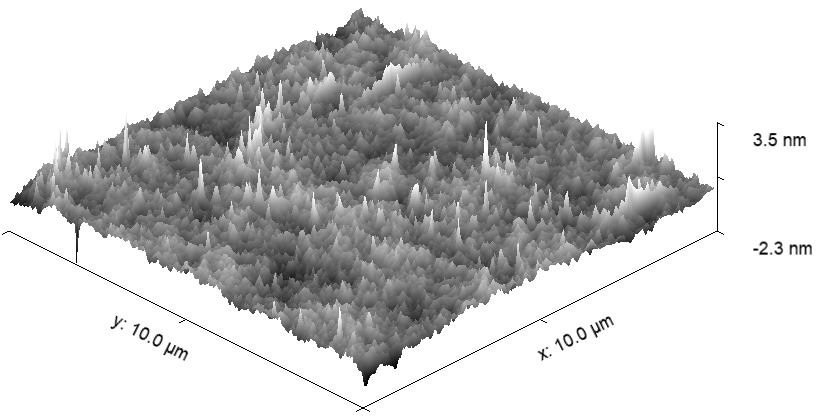
\includegraphics[scale=0.5]{source/stamp_rms}
	\caption{A ten by ten micrometer AFM scan of the surface near the tip of the glass stamp. Measurements taken at different locations yielded similar looking results.}
\end{figure}
Multiple measurements also were conducted on a flat portion of cured but not stamped OrmoComp polymer. To produce this sample the steps described in \autoref{ChapCoverslipPreparation} were followed. The result for the polymer was a \textit{mean} RMS of $0.326\nm$ with a \textit{standard deviation} of $0.01\nm$ (forward and backward measurements have been included in this calculation). The roughness of the stamp and the polymer are therefore very similar.\\
From these measurements we were able to conclude that the material properties of the stamps and the polymer used as imprinting medium both meet the specifications ($\si{RMS}<0.6\nm$). 

\begin{figure}[H]
	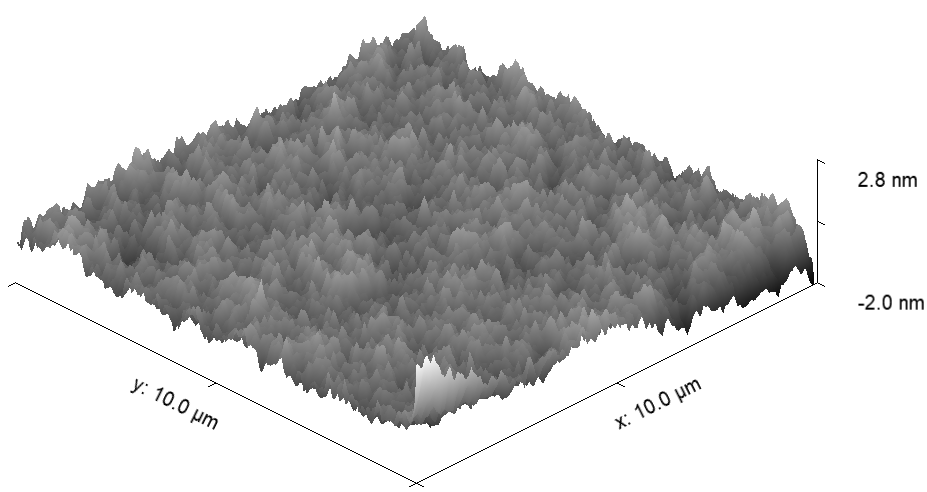
\includegraphics[scale=0.5]{source/OrmoComp_rms}
	\caption{A ten by ten micrometer AFM scan of the OrmoComp surface. Without any imprinting it can be seen that the surface of the polymer is very smooth. Other measurements yielded a similar picture.}
\end{figure}

\section{Mirror fabrication}\label{ChapMirrorFab}
Previously, we looked at the requirements that the materials involved in the process have to fulfil and how good the stamps are that we use for the mirror fabrication. Now we turn our attention at the mirrors that were actually fabricated while using this process. In \autoref{ChapGrinding} we have seen that the mirrors are ill-dimensioned, making the grinding step necessary. In this section we will look at various methods that were used to do the imprinting. These different methods were used to rule out imprecise control of the stamp as the cause of the ill-dimensioned mirrors.

\subsection{Tip station imprinting}
The first method used for imprinting involved a tip station consisting of an optical microscope and a baseplate with a micrometer screw and a pedestal to put the coverslip with the polymer layer onto. To see how close the stamp is to the polymer surface a tilted mirror was used to look sideways onto the sample (see \autoref{fig:TipStation}). To do the imprinting the procedure is to lower the stamp as close as possible to the surface until contact is made but without going into the material. From \autoref{table:CalcMirrorData} we know how deep the mirror has to be in order to match the diameter we aim for. This depth is then achieved by turning the screw accordingly. After that a UV light (US460 Lightpen) is used to cure the still fluid polymer.\\
None of the mirrors produced using this method had the required diameter of $200\um$ but rather a diameter of about $800\um$.  At the beginning it was unclear wherein the problem lies. One assumption was that the micrometer screw together with visual feedback are not precise enough for imprinting the mirrors. As it turned out this was not in fact the case. However, for this reason an alternative approach was tested. In the end, the polymer creeping up the stamp during imprinting was identified as the cause of the problem.

\begin{figure}[H]
	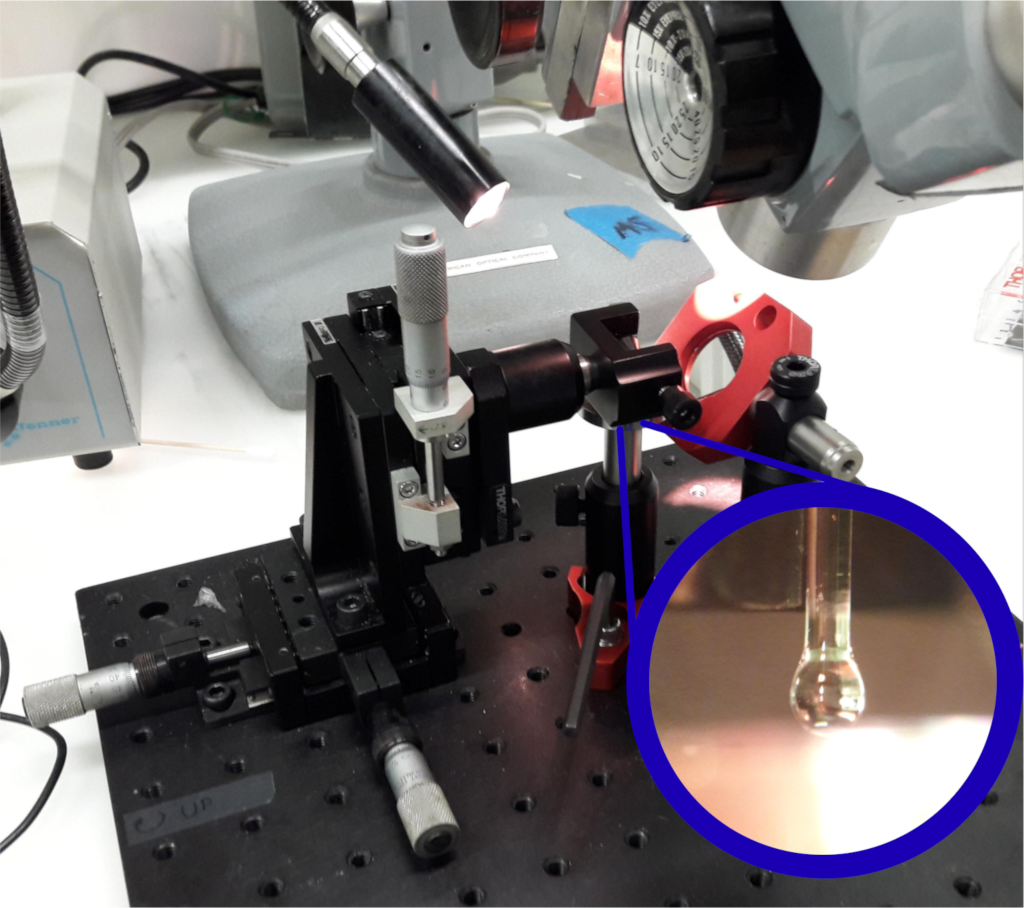
\includegraphics[scale=1]{source/tip_station_compressed}
	\caption{The micrometer screw controls the height of the glass stamp. With the microscope that is directed at the tilted mirror next to the pedestal, the distance of the stamp to the polymer can be seen.}
	\label{fig:TipStation}
\end{figure}

\begin{figure}[H]
	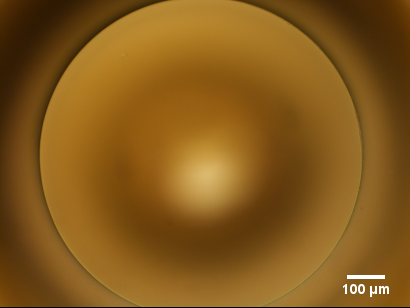
\includegraphics[scale=0.6]{source/mirror_too_large}
	\caption{All mirrors fabricated ended up having a diameter which was too large (approximately $800\um$, the aim was $200\um$). As it turned out this was due to the polymer creeping up the glass stamp during imprinting.}
\end{figure}

\subsection{Inverted microscope imprinting}
The suspicion that the microscope looking sideways onto the polymer surface is an insufficient tool to control the imprinting depth of the stamp into the polymer led to a different approach. In this approach the sample is placed over a microscope which then is focused to the surface. To estimate how far away the stamp is, the focus is adjusted to the tip of the stamp.

\begin{figure}[H]
	\includesvg[scale=0.65]{source/inverted_microscope}
	\caption{This method uses an upside-down microscope mounted below the sample to estimate the distance of the stamp to the polymer surface. Moving the setup up and down allows focusing on different objects. With the objective used, a resolution on the nanometer-scale is possible.}
\end{figure}
In our lab environment this setup required a lot of preparation and took a lot of time to implement. Thanks to the objective which was used for the focusing, a resolution on the nanometer-scale is possible. Nevertheless, after completing the imprinting with this method the diameter was still too large. However, through the microscope it was clearly visible that the polymer was in fact creeping up the glass stamp, therefore lending evidence to the conclusion that the problem is not the control of the stamp.

\subsection{Grinding and results}
The fact that all imprinted mirrors were too deep and had a diameter too large for the utilization in a microcavity means that sandpaper had to be used to dimension the mirrors properly. The consequence of using this sandpaper method is that it requires a lot of attention not to remove too much material. \autoref{table:MirrorRMSResults} shows the RMS values extracted from the mirrors where grinding and subsequent cleaning was successful.

\begin{table}[H]
	\begin{tabular}{cccc}
	\hline
	\textbf{forward $[\nm]$} & \textbf{forward* $[\nm]$} & \textbf{backward $[\nm]$} & \textbf{backward* $[\nm]$} \\
	\hline
	2.17 & 2.03 & 1.74 & 1.60 \\
	1.72 & 1.37 & 1.68 & 1.34 \\
	1.87 & 1.71 & 1.86 & 1.70 \\
	2.08 & 1.91 & 2.11 & 1.94 \\
	\hline
	\end{tabular}
	\caption{The table shows the RMS values of the mirrors where grinding and cleaning was successful. The columns show if the values were acquired during a forward or a backward scan with the AFM. The (*) marks that grains and measurement artefacts were removed with post processing software (Gwyddion 2.52).}
	\label{table:MirrorRMSResults}
\end{table}

In the end we were only able to produce four mirrors that did not break during the last two processing steps. In summary it can be said that the mean RMS over the mirrors is $\si{RMS}=1.90\nm$ and if we remove measurement artifacts and grains by software we have $\si{RMS}=1.70\nm$. These results show that the mirrors do not meet the surface roughness requirement of $\si{RMS}<0.6\nm$. This means that they would lead to losses of around $100$ to $200\ppm$ if used in a cavity.

\begin{figure}[H]
	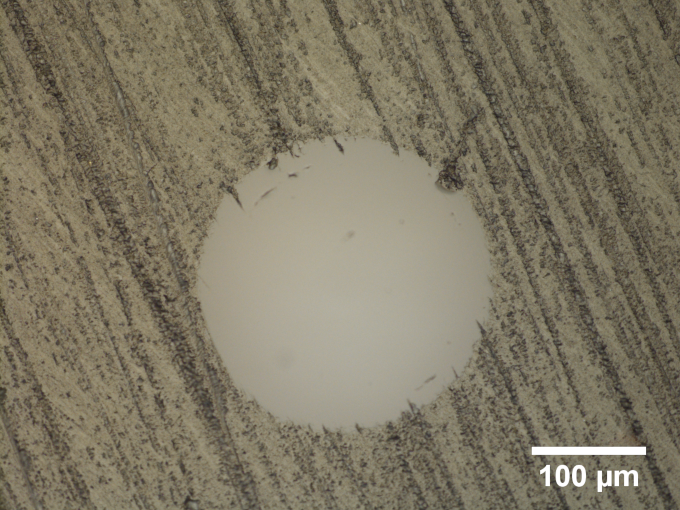
\includegraphics[scale=1]{source/grinded_cleaned_compressed}
	\caption{A cavity mirror after grinding and cleaning. It can be seen that the outer ring of the mirror has some scratches in it. The scratches were probably caused by the rough sandpaper ($30\um$).}
\end{figure}

\section{Challanges}\label{ChapProblems}
During the entirety of this chapter we have looked at the results of all the different fabrication processes that make up the content of this project. While we were able to implement stable processes for the stamp fabrication, silanization and automated measurements procedures, other goals were not reached. Most importantly it was not possible during the course of this project to produce mirrors with a smooth enough surface to send them in for coating.\\
To analyze this problem, measurements of the different materials were taken and the glass stamps as well as the OrmoComp polymer were ruled out as direct causes of the roughness problem. A more likely source of the problem are the last steps of the process: Grinding and cleaning. Especially grinding cannot be controlled very well and has caused a lot of mirrors to break during fabrication. Since the depth of the mirrors was estimated to be around $3\um$ which is also the roughness of the smoothest sandpaper used while grinding, we see that there is not much room for error. The cleaning process also bares a high risk. If the optical cleaning liquid is not removed carefully, the entire mirror can be ripped off or be damaged otherwise. Those arguments are strong indicators that the last two steps are the cause for the roughness problem but there is no conclusive evidence yet and further tests will be necessary.

\section{Possible solutions/improvements}\label{ChapSolutions}
In the last section we have identified the grinding and cleaning steps as the likely cause for the surface roughness which is too high in the fabricated mirrors. The most obvious improvement would be to just omit both processing steps altogether. We have to understand why the mirrors get too wide and therefore too deep. As discussed in \autoref{ChapMirrorFab}, the control of the stamp during imprinting was ruled out as the problem. Another source of the problem could be the silanization process as it may not work as intended. After calling Microresist, the manufacturer of OrmoComp we found out that the creeping is an intended effect of the polymer and ensures that every detail of the stamp is captured properly. According to Microresist this has nothing to do with silanization.
With this knowledge it was possible to develop a new idea for the imprinting process. Since the way OrmoComp is supposed to be used is with arrays of stamps where a "ceiling" limits the height the polymer can lift itself up we also need a ceiling or walls in our method (see \autoref{fig:newIdea}).

\begin{figure}[H]
	\includesvg[scale=0.45]{source/new_stamp_idea}
	\caption{Since OrmoComp tries to capture every detail by creeping up the stamp the solution to prohibit this behaviour is to add walls which retain the polymer. By adding the glass coverslip to the stamp with a hole that has exactly the diameter which is needed for the mirror ($200\um$) the mirror wont get too large and neither too deep.}
	\label{fig:newIdea}
\end{figure}

To only get the mirror without the excess material shown in \autoref{fig:newIdea}, a spin coater can be used. After the polymer has been put into the mould it can be cured. The question remains if the mirror will stay inside of the coverslip if the stamp is removed or if it comes out with the stamp. In both cases the retrieval of the mirror should be possible without much difficulties.\\
The challenge of this method is how to get a hole with the correct diameter into the coverslip. One method could be to use ultra-short laser pulse ablation to create the hole.  Unfortunately, due to the lack of equipment and time constraints we were not able to test this method. As a first step, tests were conducted with steel plates and holes with $1\mm$ diameter. These tests showed that the OrmoComp can successfully be restricted in its expansion.